\documentclass[14pt,a4paper]{extarticle}

\usepackage{fontspec}
\usepackage{polyglossia}
\setmainlanguage{russian}
\setotherlanguage{english}
\setmainfont{Times New Roman}
\newfontfamily\cyrillicfont{Times New Roman}
\setmonofont{Courier New}
\newfontfamily\cyrillicfonttt{Courier New}

\usepackage{geometry}
\geometry{left=30mm,right=15mm,top=20mm,bottom=20mm}
\usepackage{setspace}
\onehalfspacing
\usepackage{indentfirst}
\setlength{\parindent}{1.25cm}
\usepackage{graphicx}
\usepackage{float}
\usepackage{booktabs}
\usepackage{array}
\usepackage{longtable}
\usepackage{tabularx}
\usepackage{xcolor}
\usepackage{listings}
\usepackage{caption}
\usepackage{subcaption}
\usepackage{hyperref}
\usepackage{tikz}
\usetikzlibrary{arrows.meta,positioning,fit,calc,shapes.geometric,backgrounds}

\graphicspath{{assets/}}
\hypersetup{hidelinks}

\lstdefinestyle{code}{
    basicstyle=\ttfamily\small,
    breaklines=true,
    frame=single,
    columns=fullflexible,
    keepspaces=true,
    showstringspaces=false,
    backgroundcolor=\color{gray!5}
}
\lstdefinelanguage{json}{
    basicstyle=\ttfamily\small,
    string=[s]{"}{"},
    stringstyle=\color{blue!50!black},
    comment=[l]{:},
    commentstyle=\color{black},
    morecomment=[l]{//},
    moredelim=**[is][\color{black}]{@}{@}
}
\lstset{style=code}

\captionsetup{labelsep=endash}

\begin{document}

\begin{titlepage}
\thispagestyle{plain}
\begin{center}
    {\bfseries МИНИСТЕРСТВО ЦИФРОВОГО РАЗВИТИЯ,\\
    СВЯЗИ И МАССОВЫХ КОММУНИКАЦИЙ\\
    РОССИЙСКОЙ ФЕДЕРАЦИИ}\\[1.0cm]

    Федеральное государственное бюджетное образовательное\\
    учреждение высшего образования\\[0.8cm]

    Сибирский государственный университет телекоммуникаций и\\
    информатики\\[0.8cm]

    Кафедра телекоммуникационных систем и вычислительных\\
    средств (ТС и ВС)\\[4.0cm]

    {\bfseries\Large РАСЧЕТНО-ГРАФИЧЕСКАЯ РАБОТА}\\[0.35cm]
    {\bfseries Визуальное программирование и человеко -- машинное\\
    взаимодействие}\\[2.0cm]
\end{center}

\begin{flushright}
    Выполнил: студент гр. ИКС-431\\
    Антропов Д. С.\\
    Проверил:\\
    \textit{Старший преподаватель}\\
    Ахпашев Р. В.
\end{flushright}

\vfill
\begin{center}
    Новосибирск, 2026
\end{center}
\end{titlepage}

\tableofcontents
\newpage

\section{Введение}

В рамках расчетно-графической работы был разработан программно-аппаратный комплекс для сбора, передачи, хранения и визуализации параметров мобильной сети. Комплекс состоит из Android-приложения и настольного backend-приложения на языке C++. Смартфон выступает в роли измерительного устройства: он получает координаты, параметры базовых станций, значения уровня радиосигнала и статистику сетевого трафика. Desktop-приложение принимает данные по сети, сохраняет их в файл и базу данных, строит графики, отображает маршрут на OpenStreetMap и формирует тепловые карты.

Практическая часть проекта объединяет задания по работе с местоположением смартфона, сокетами, ZeroMQ, сервисами Android, backend-сервером на C++, PostgreSQL, графическим интерфейсом ImGui/ImPlot, картографической подложкой OSM и алгоритмом построения heatmap методом обратных взвешенных расстояний. Основная цель проекта --- получить сквозной цикл обработки телеметрии: от получения измерения на смартфоне до анализа результата на компьютере.

Разработанное Android-приложение имеет основное меню, из которого пользователь может перейти к модулям калькулятора, медиаплеера и монитора. Для данной работы ключевым является модуль <<Монитор>>, который запускает foreground-service, получает координаты и данные сотовой сети, записывает накопленные измерения в JSON-файл либо отправляет их на сервер. Внешний вид главного меню приложения показан на рисунке~\ref{fig:android-menu}.

\begin{figure}[H]
    \centering
    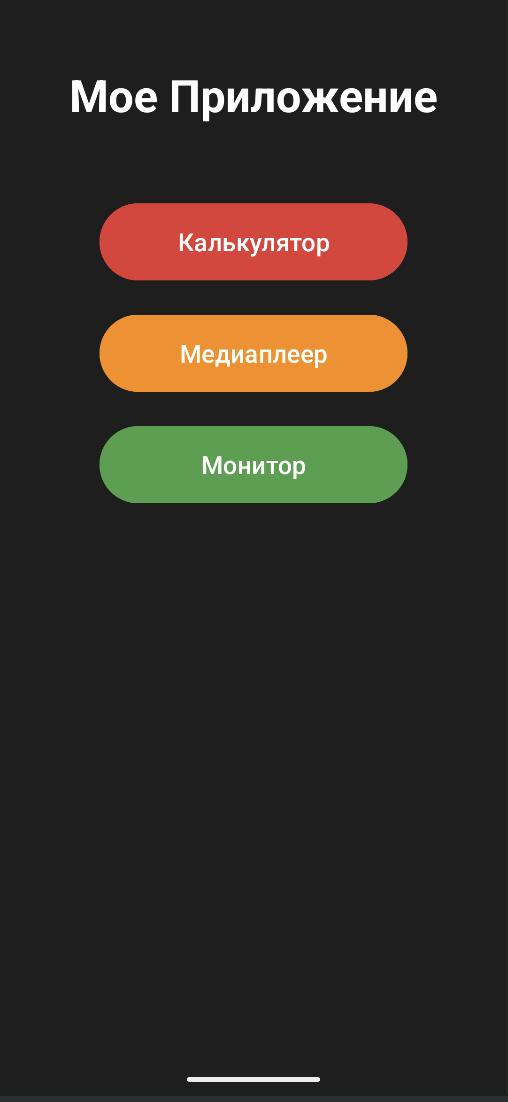
\includegraphics[height=0.72\textheight]{android_menu.png}
    \caption{Главное меню Android-приложения}
    \label{fig:android-menu}
\end{figure}

Backend-приложение называется Phone Monitor. Оно принимает JSON-пакеты от Android-клиента через ZeroMQ, парсит их, обновляет общую структуру данных, сохраняет информацию в PostgreSQL и отображает измерения в графическом интерфейсе. На рисунке~\ref{fig:backend-heatmap} показана вкладка построения тепловой карты RSRP на фоне OpenStreetMap.

\begin{figure}[H]
    \centering
    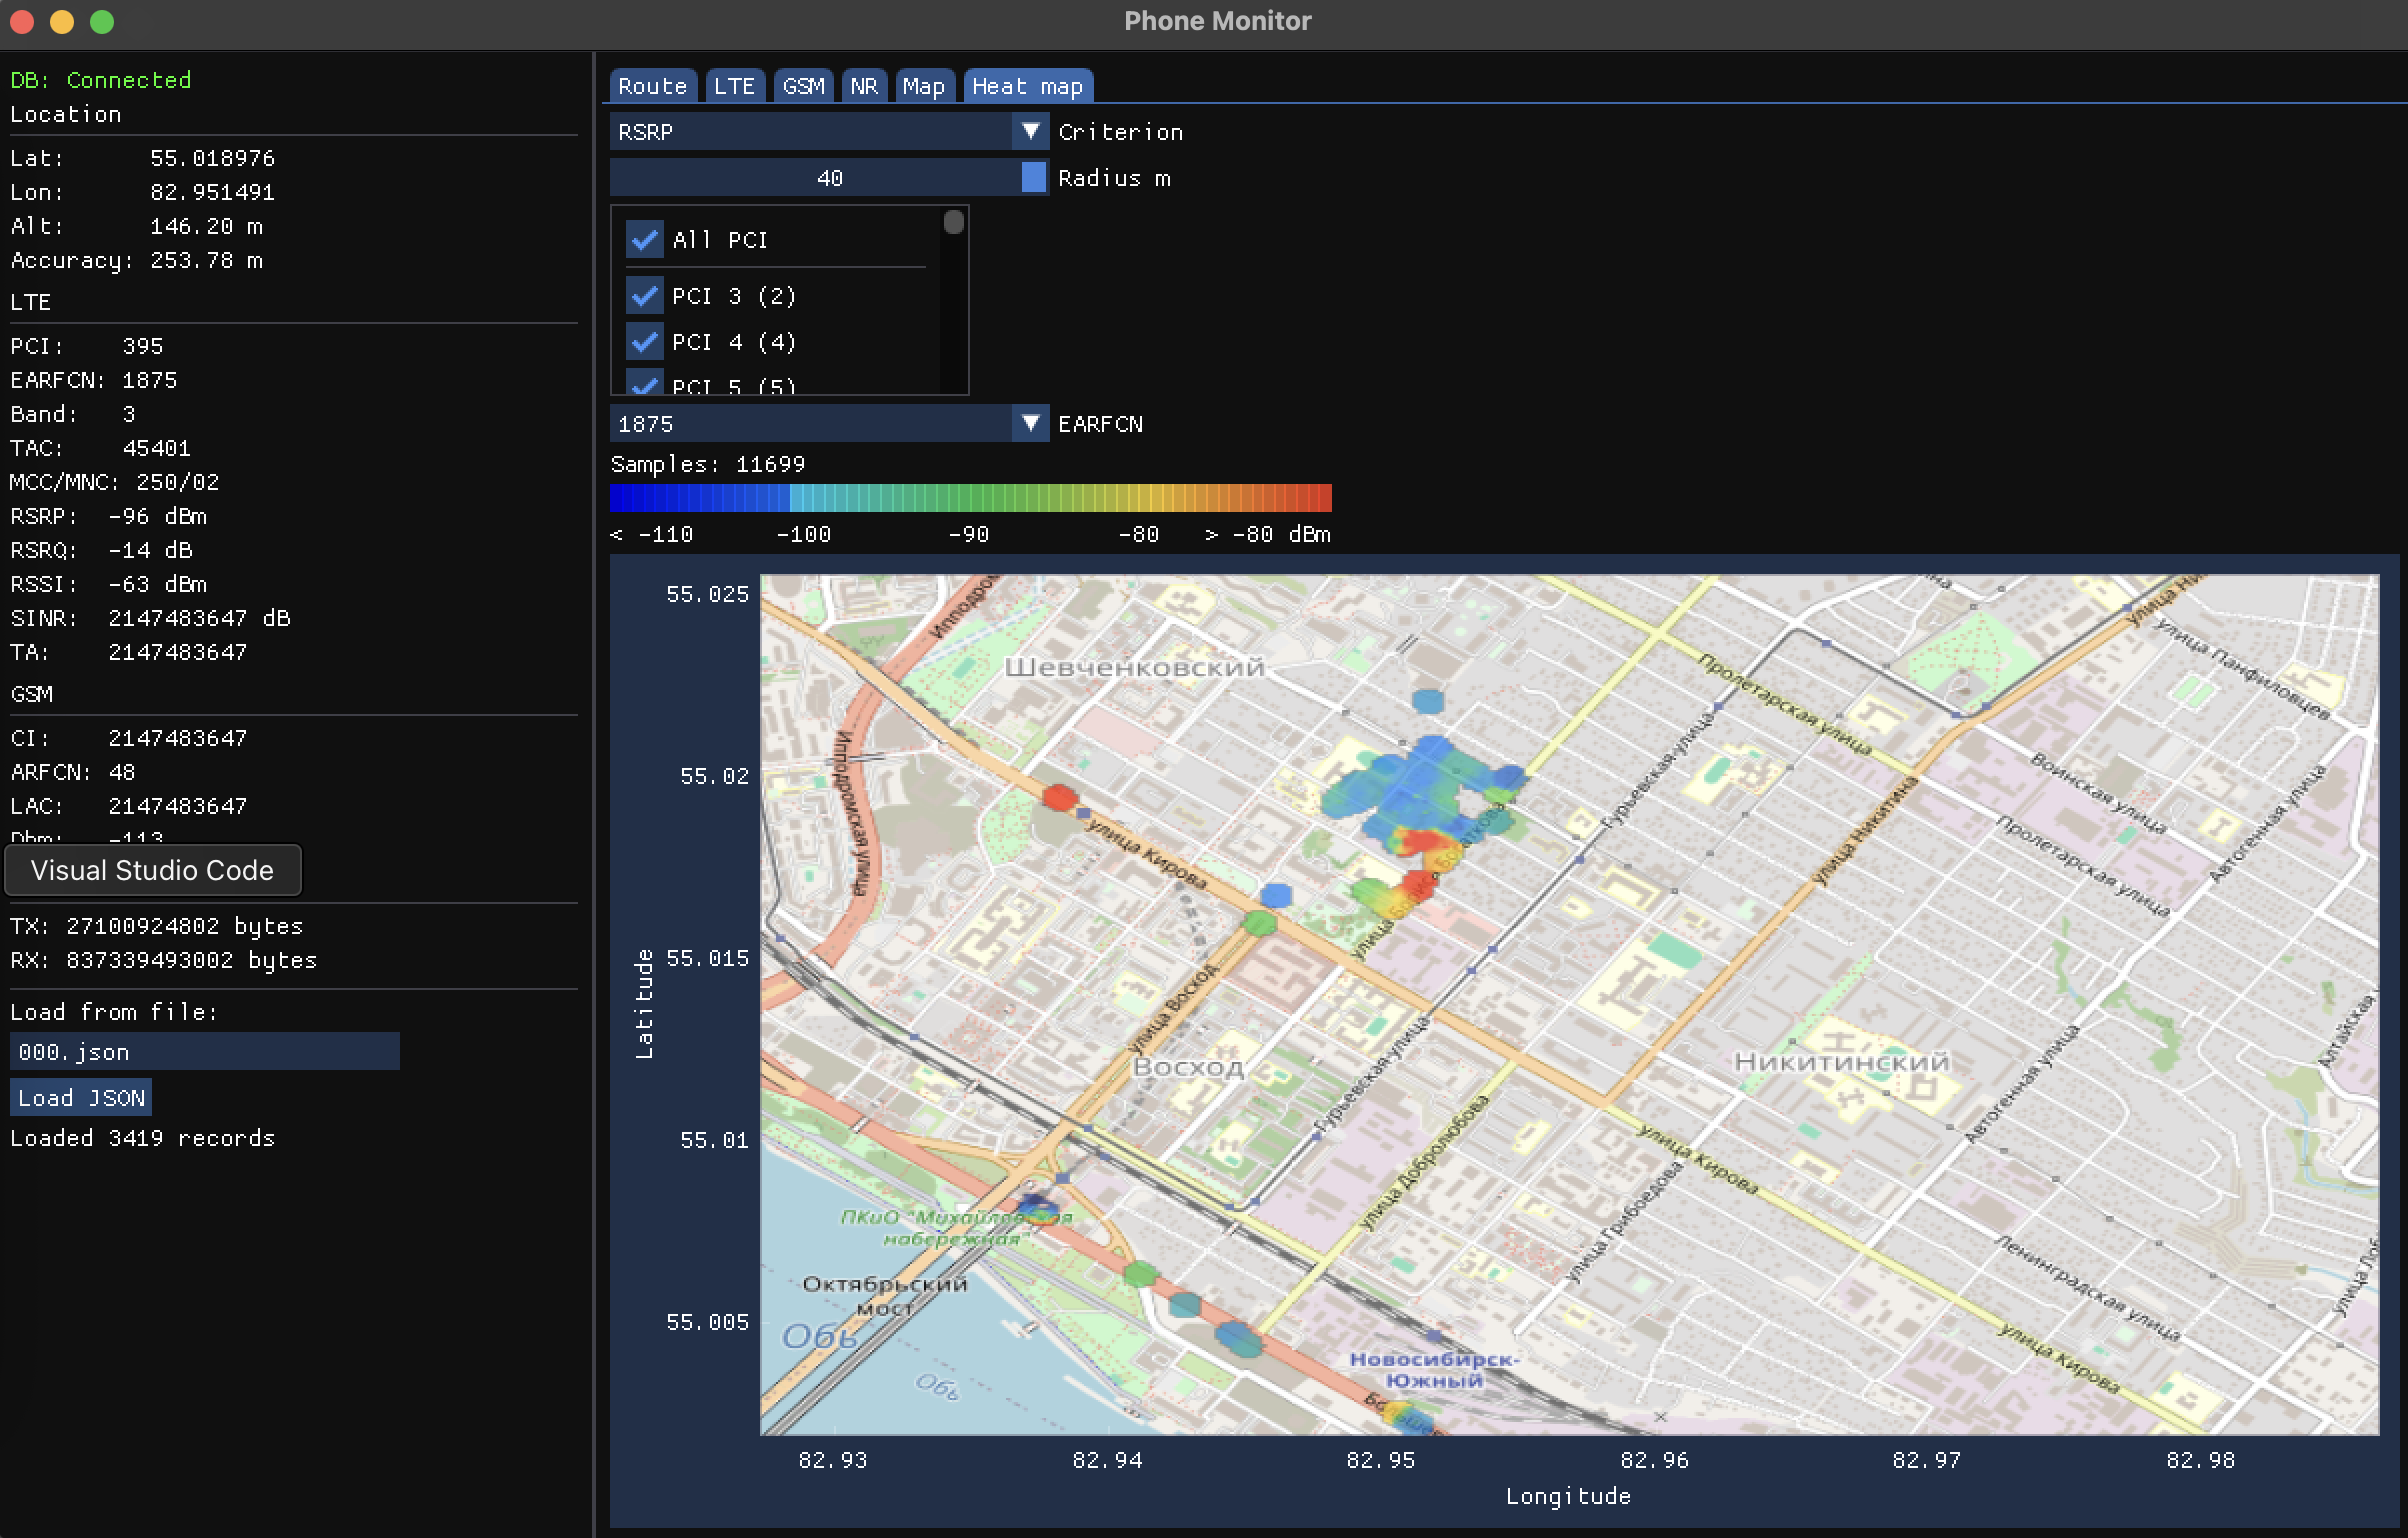
\includegraphics[width=\textwidth]{backend_heatmap.png}
    \caption{Desktop-интерфейс Phone Monitor с тепловой картой RSRP}
    \label{fig:backend-heatmap}
\end{figure}

\section{Общая архитектура проекта}

Комплекс построен по клиент-серверной модели. Android-приложение собирает телеметрию и формирует JSON-сообщение. Сообщение передается на компьютер по TCP с использованием паттерна ZeroMQ REQ/REP. Backend-сервер принимает пакет, отправляет ответ клиенту, сохраняет исходный JSON и обновляет состояние графического интерфейса.

В проекте используются следующие основные компоненты:
\begin{itemize}
    \item Android-приложение на Kotlin;
    \item foreground-service для фонового сбора координат и параметров сети;
    \item ZeroMQ как транспортный слой между смартфоном и компьютером;
    \item C++20 backend-сервер;
    \item PostgreSQL для долговременного хранения измерений;
    \item ImGui и ImPlot для графического интерфейса и графиков;
    \item OpenStreetMap и libcurl для загрузки тайлов карты;
    \item алгоритм IDW для генерации тепловой карты.
\end{itemize}

\subsection{Схема программно-аппаратного комплекса}

На рисунке~\ref{fig:architecture} представлена схема разработанного проекта. В верхней части находится Android-приложение, которое собирает GPS, CellInfo и traffic-данные. В центральной части расположено C++ backend-приложение, где выделены серверный поток, GUI-поток, модуль карты, модуль тепловой карты и база данных. В нижней части показано хранение данных в PostgreSQL и файловом кэше.

\begin{figure}[H]
\centering
\begin{tikzpicture}[
    font=\small,
    node distance=5mm and 4mm,
    % ---- стили ----
    blk/.style={
        rounded corners=3pt, draw=#1!70!black, fill=#1!15,
        thick, align=center, minimum height=10mm, minimum width=32mm,
        text width=30mm
    },
    hdr/.style={
        rounded corners=4pt, draw=#1!70!black, fill=#1!55!black,
        very thick, align=center, text=white,
        minimum width=32mm, text width=30mm, minimum height=8mm
    },
    busnode/.style={
        rounded corners=3pt, draw=black!60, fill=black!75,
        text=white, thick, align=center,
        minimum height=10mm, minimum width=90mm, text width=88mm
    },
    storebox/.style={
        rounded corners=3pt, draw=#1!70!black, fill=#1!10,
        thick, align=center, minimum height=10mm,
        minimum width=38mm, text width=36mm
    },
    arr/.style={-{Latex[length=2.5mm,width=1.8mm]}, thick, draw=black!55},
    grp/.style={rounded corners=5pt, draw=#1!60!black, fill=#1!6, very thick}
]

%% ======================================================
%% БЛОК 1: Android
%% ======================================================
\node[hdr=teal, minimum width=130mm, text width=128mm] (ahdr)
    {Android-приложение: foreground service, сбор телеметрии};

\node[blk=teal, below=6mm of ahdr, xshift=-46mm] (gps)
    {GPS\\lat, lon, alt};
\node[blk=teal, right=4mm of gps] (cell)
    {CellInfo\\LTE / NR / GSM};
\node[blk=teal, right=4mm of cell] (sig)
    {Сигнал\\RSRP, RSRQ, RSSI};
\node[blk=teal, right=4mm of sig] (chan)
    {Канал\\EARFCN, PCI, TAC};

\begin{scope}[on background layer]
\node[grp=teal, fit=(ahdr)(gps)(cell)(sig)(chan), inner sep=4mm] (android) {};
\end{scope}

%% ======================================================
%% Шина ZeroMQ
%% ======================================================
\node[busnode, below=8mm of android.south] (zmq)
    {ZMQ REQ/REP + TCP :5555 \quad JSON: location, lte, gsm, nr, traffic};

\draw[arr] (android.south) -- (zmq.north);

%% ======================================================
%% БЛОК 2: C++ Backend — 4 колонки
%% ======================================================
\node[hdr=violet, minimum width=130mm, text width=128mm,
      below=8mm of zmq.south] (bhdr)
    {C++ Backend: SDL2 + OpenGL 3.3 + ImGui + ImPlot};

% Колонка A: сервер / парсер
\node[blk=violet, below=7mm of bhdr, xshift=-46mm] (main)
    {main.cpp\\запуск потоков};
\node[blk=violet, below=5mm of main] (server)
    {server.cpp\\ZMQ сервер};
\node[blk=violet, below=5mm of server] (parser)
    {json\_parser.cpp\\разбор пакета};

% Колонка B: GUI / карта
\node[blk=blue!80!cyan, below=7mm of bhdr, xshift=-13mm] (gui)
    {gui.cpp\\окна и графики};
\node[blk=blue!80!cyan, below=5mm of gui] (map)
    {osm\_map.cpp\\Web Mercator};
\node[blk=blue!80!cyan, below=5mm of map] (curl)
    {curl\_func.cpp\\загрузка OSM};

% Колонка C: тепловая карта
\node[blk=red!80, below=7mm of bhdr, xshift=20mm] (heat)
    {heatmap.cpp\\IDW heatmap};
\node[blk=red!80, below=5mm of heat] (criteria)
    {RSRP / RSRQ / RSSI\\Altitude, PCI};

% Колонка D: БД / рендер
\node[blk=orange!90!red, below=7mm of bhdr, xshift=53mm] (db)
    {database.cpp\\libpq};
\node[blk=gray!70, below=5mm of db] (gl)
    {OpenGL поток\\рендер};

\begin{scope}[on background layer]
\node[grp=violet,
      fit=(bhdr)(main)(server)(parser)(gui)(map)(curl)(heat)(criteria)(db)(gl),
      inner sep=4mm] (backend) {};
\end{scope}

% Стрелки внутри backend
\draw[arr] (zmq.south) -- (zmq.south |- server.north) -- (server.north);
\draw[arr] (main)   -- (server);
\draw[arr] (server) -- (parser);
\draw[arr] (gui)    -- (map);
\draw[arr] (map)    -- (curl);
\draw[arr] (heat)   -- (criteria);

%% ======================================================
%% БЛОК 3: Хранение данных
%% ======================================================
\node[storebox=brown, below=10mm of backend.south, xshift=-35mm] (pg)
    {PostgreSQL\\phone\_monitor\\таблица telemetry};
\node[storebox=brown, right=6mm of pg] (jsonf)
    {JSON-файлы\\drive\_data.json\\000.json};
\node[storebox=brown, right=6mm of jsonf] (cache)
    {Файловый кэш\\OSM и heatmap PNG};

\begin{scope}[on background layer]
\node[grp=brown, fit=(pg)(jsonf)(cache), inner sep=4mm,
      label={[brown!60!black, font=\small\bfseries]above:Хранение данных}]
      (storage) {};
\end{scope}

% Стрелки к хранилищу
\draw[arr] (db.south)     |- (pg.west);
\draw[arr] (parser.south) |- (jsonf.west);
\draw[arr] (curl.south)   |- (cache.west);
\draw[arr] (criteria.south) |- (cache.east);

\end{tikzpicture}
\caption{Архитектура программно-аппаратного комплекса}
\label{fig:architecture}
\end{figure}

\section{Теоретическая часть}

\subsection{Координаты LLA}

В задаче мониторинга мобильной сети важны координаты точки измерения. В проекте используется представление LLA: latitude, longitude, altitude.

Latitude --- географическая широта. Она показывает положение точки относительно экватора и измеряется в градусах. Диапазон широты ограничен значениями от $-90^\circ$ до $+90^\circ$: отрицательные значения соответствуют южному полушарию, положительные --- северному.

Longitude --- географическая долгота. Она показывает положение точки относительно нулевого меридиана и также измеряется в градусах. Диапазон долготы составляет от $-180^\circ$ до $+180^\circ$: отрицательные значения соответствуют западной долготе, положительные --- восточной.

Altitude --- высота над уровнем моря. В Android-классе \texttt{Location} высота возвращается в метрах. Значение зависит от источника определения местоположения: GPS, Wi-Fi, сотовые сети или их комбинация. Кроме координат Android также предоставляет accuracy --- оценку точности в метрах.

В программе координаты используются не только для вывода пользователю, но и для построения маршрута, привязки измерений к карте и интерполяции тепловой карты. Для каждого JSON-пакета сохраняются широта, долгота, высота, точность и время измерения.

\subsection{Unix Epoch Time}

Unix Epoch Time --- это способ представления времени как количества миллисекунд или секунд, прошедших с 00:00:00 UTC 1 января 1970 года. В Android для получения текущего времени используется метод \texttt{System.currentTimeMillis()}, который возвращает число миллисекунд с начала эпохи Unix.

В мобильных телефонах системное время может синхронизироваться по сети оператора, через NTP и по данным GNSS. В спутниковых системах навигации используется собственная шкала времени, отличающаяся от гражданского UTC, поэтому приемник выполняет пересчет. Точность времени в смартфоне зависит от источника синхронизации, качества приема спутникового сигнала, задержек сети и алгоритмов операционной системы.

\subsection{GSM, LTE и NR}

GSM --- цифровой стандарт мобильной связи второго поколения. В проекте для GSM сохраняются идентификатор соты, ARFCN, LAC, MCC, MNC и уровень сигнала в dBm. Эти данные позволяют определить, с какой сотой взаимодействовал телефон и насколько устойчивым был прием.

LTE --- стандарт четвертого поколения, использующий OFDMA в нисходящем канале и SC-FDMA в восходящем. Для LTE важны параметры \texttt{PCI}, \texttt{EARFCN}, \texttt{TAC}, \texttt{Band}, \texttt{RSRP}, \texttt{RSRQ}, \texttt{RSSI}, \texttt{RSSNR} и Timing Advance. В drive-test анализе особенно важны RSRP и RSRQ, потому что они характеризуют покрытие и качество радиоканала.

NR --- стандарт пятого поколения. В Android для NR доступны \texttt{NCI}, \texttt{PCI}, \texttt{NRARFCN}, \texttt{TAC}, \texttt{SS-RSRP}, \texttt{SS-RSRQ}, \texttt{SS-SINR}. В проекте эти значения также включены в JSON и могут быть сохранены на стороне backend.

\subsection{Критерии качества радиосигнала}

RSSI показывает общий уровень принятой мощности в полосе канала. Этот параметр включает полезный сигнал, шум и интерференцию, поэтому сам по себе не всегда точно отражает качество LTE-соединения.

RSRP --- Reference Signal Received Power. Это мощность опорных сигналов LTE, измеряемая в dBm. RSRP используется для оценки покрытия. Чем ближе значение к нулю, тем сильнее сигнал. Например, $-80$ dBm лучше, чем $-105$ dBm.

RSRQ --- Reference Signal Received Quality. Этот параметр учитывает отношение RSRP к RSSI и позволяет оценивать качество приема с учетом загруженности и помех.

В проекте для тепловой карты RSRP используются следующие интервалы:

\begin{table}[H]
\centering
\caption{Критерии качества RSRP}
\begin{tabularx}{\textwidth}{>{\bfseries}l l X}
\toprule
Категория & Диапазон & Интерпретация \\
\midrule
Excellent & $>-80$ dBm & сильный сигнал, максимальные скорости передачи данных \\
Good & $-80 \ldots -90$ dBm & надежная работа соединения \\
Fair/Marginal & $-90 \ldots -100$ dBm & соединение работоспособно, но возможны просадки скорости \\
Poor/Weak & $-100 \ldots -110$ dBm & возможны обрывы и низкая скорость \\
No Signal/Unusable & $<-110$ dBm & соединение часто недоступно \\
\bottomrule
\end{tabularx}
\end{table}

\section{Android-приложение}

\subsection{Назначение и структура}

Android-приложение находится в директории \texttt{/Users/m1/Desktop/work/android}. Основной пакет приложения --- \texttt{com.example.myapplication}. В проекте реализованы несколько Activity: главное меню, калькулятор, медиаплеер, модуль местоположения, модуль тестовой передачи ZMQ и модуль CellInfo.

Ключевые файлы Android-части:
\begin{itemize}
    \item \texttt{MainActivity.kt} --- главное меню приложения;
    \item \texttt{LocationActivity.kt} --- интерфейс запуска мониторинга;
    \item \texttt{MonitorService} --- foreground-service для фонового сбора данных;
    \item \texttt{CellInfoActivity.kt} --- сбор CellInfo и отправка JSON на сервер;
    \item \texttt{SocketsZmqActivity.kt} --- простая проверка ZeroMQ REQ/REP;
    \item \texttt{AndroidManifest.xml} --- разрешения и регистрация Activity/Service.
\end{itemize}

В манифесте запрошены разрешения на доступ к интернету, точному и приблизительному местоположению, фоновой геолокации, состоянию телефона, статистике приложений и foreground-service. Это соответствует требованиям практик: приложение может получать координаты, параметры сотовой сети и работать в фоне.

\subsection{Получение местоположения}

Для получения координат используется \texttt{LocationManager}. В сервисе запускаются обновления от \texttt{GPS\_PROVIDER} и \texttt{NETWORK\_PROVIDER}. При поступлении нового значения вызывается \texttt{onLocationChanged()}, где сохраняется последнее известное местоположение. Далее каждые пять секунд сервис формирует JSON-пакет.

Фрагмент логики формирования объекта \texttt{location}:

\begin{lstlisting}[language=Java,caption={Формирование блока location в Android-сервисе}]
val loc = lastLocation
val t = System.currentTimeMillis()
if (loc != null)
    sb.append("\"location\":{\"latitude\":${loc.latitude},\"longitude\":${loc.longitude},\"altitude\":${loc.altitude},\"accuracy\":${loc.accuracy},\"time\":$t}")
else
    sb.append("\"location\":{\"latitude\":0,\"longitude\":0,\"altitude\":0,\"accuracy\":0,\"time\":$t}")
\end{lstlisting}

Для пользователя предусмотрено два режима работы. В онлайн-режиме данные отправляются на сервер. В офлайн-режиме JSON-пакеты записываются в файл \texttt{drive\_data.json}, что удобно для drive-test, когда сервер временно недоступен.

\subsection{Сбор параметров мобильной сети}

Для получения информации о сотах используется \texttt{TelephonyManager.allCellInfo}. В проекте обрабатываются LTE, GSM и NR-соты.

Для LTE сохраняются:
\begin{itemize}
    \item \texttt{band}, \texttt{ci}, \texttt{earfcn}, \texttt{mcc}, \texttt{mnc};
    \item \texttt{pci}, \texttt{tac};
    \item \texttt{asu}, \texttt{cqi}, \texttt{rsrp}, \texttt{rsrq}, \texttt{rssi};
    \item \texttt{rssnr}, \texttt{ta}.
\end{itemize}

Для GSM сохраняются \texttt{ci}, \texttt{bsic}, \texttt{arfcn}, \texttt{lac}, \texttt{mcc}, \texttt{mnc}, \texttt{dbm}, \texttt{rssi} и \texttt{ta}. Для NR сохраняются \texttt{band}, \texttt{nci}, \texttt{pci}, \texttt{nrarfcn}, \texttt{tac}, \texttt{mcc}, \texttt{mnc}, \texttt{ss\_rsrp}, \texttt{ss\_rsrq}, \texttt{ss\_sinr}.

\subsection{Сбор сетевого трафика}

Дополнительно приложение собирает суммарный объем переданных и принятых данных через \texttt{TrafficStats}. Для определения приложений с высоким потреблением трафика используется \texttt{NetworkStatsManager}. Сначала собирается статистика по установленным приложениям, затем вычисляются среднее значение и стандартное отклонение. В список попадают приложения, находящиеся выше порога $\mu + 2\sigma$.

Такой подход позволяет не выводить весь список приложений, а оставить только наиболее заметных потребителей трафика. Это полезно при анализе drive-test, потому что передача данных по сети зависит не только от качества радиосигнала, но и от активности приложений.

\subsection{Фоновый сервис}

Класс \texttt{MonitorService} реализован как foreground-service. Это позволяет продолжать запись измерений, когда Activity не находится на экране пользователя. Сервис запускает уведомление, получает обновления координат, формирует JSON и либо пишет его в файл, либо отправляет на backend.

Сервис использует корутины:
\begin{lstlisting}[language=Java,caption={Цикл периодической отправки данных}]
serviceScope.launch {
    while (isActive) {
        delay(5000)
        val json = buildJson()
        if (offline) {
            saveToFile(json)
            broadcast("Записано в файл", json)
        } else {
            broadcast("Отправка...", json)
            sendToServer(json)
        }
    }
}
\end{lstlisting}

Для связи Activity и Service используется broadcast. Activity получает статус и последний JSON-пакет, форматирует его и выводит на экран.

\subsection{Формат JSON}

Один пакет данных содержит координаты, список LTE/GSM/NR-сот и статистику трафика:

\begin{lstlisting}[language=json,caption={Пример JSON-пакета Android-приложения}]
{
  "location": {
    "latitude": 55.018976,
    "longitude": 82.951491,
    "altitude": 146.2,
    "accuracy": 253.78,
    "time": 1773768390621
  },
  "lte": [
    {
      "band": 3,
      "ci": 138245901,
      "earfcn": 1875,
      "mcc": "250",
      "mnc": "02",
      "pci": 395,
      "tac": 45401,
      "rsrp": -96,
      "rsrq": -14,
      "rssi": -63,
      "rssnr": 2147483647
    }
  ],
  "traffic": {
    "total_tx": 27100924802,
    "total_rx": 837339493002,
    "top_apps": []
  }
}
\end{lstlisting}

\section{ZeroMQ и клиент-серверное взаимодействие}

ZeroMQ используется как библиотека обмена сообщениями поверх TCP. В проекте выбран шаблон REQ/REP: клиент отправляет запрос, сервер принимает JSON и отвечает строкой подтверждения. Такой паттерн прост для отладки и подходит для периодической отправки телеметрии.

На Android создается сокет \texttt{SocketType.REQ}, который подключается к адресу \texttt{tcp://<ip>:5555}. После отправки JSON клиент ожидает ответ. Если ответ не приходит за заданный таймаут, приложение сообщает об ошибке и повторяет попытку отправки.

На стороне C++ backend работает серверный поток. Он принимает сообщения, парсит JSON, обновляет глобальную структуру телеметрии и возвращает ответ клиенту. Отдельный поток нужен для того, чтобы прием данных не блокировал интерфейс ImGui.

\section{Backend-приложение на C++}

\subsection{Структура проекта}

Backend находится в директории \texttt{/Users/m1/Desktop/visual}. Проект собирается через CMake и использует C++20. Структура исходного кода разделена по назначению:

\begin{longtable}{p{0.32\textwidth}p{0.60\textwidth}}
\caption{Основные файлы backend-приложения}\\
\toprule
Файл & Назначение \\
\midrule
\endfirsthead
\toprule
Файл & Назначение \\
\midrule
\endhead
\texttt{main.cpp} & запуск приложения, создание серверного потока и GUI \\
\texttt{server.cpp/.h} & ZeroMQ-сервер, прием JSON-пакетов \\
\texttt{gui.cpp/.h} & графический интерфейс ImGui/ImPlot \\
\texttt{json\_parser.cpp/.h} & разбор JSON и заполнение структур данных \\
\texttt{database.cpp/.h} & подключение к PostgreSQL и запись строк в таблицу \\
\texttt{osm\_map.cpp/.h} & пересчет координат в тайлы OSM, работа с картой \\
\texttt{curl\_func.cpp/.h} & загрузка PNG-тайлов через libcurl \\
\texttt{heatmap.cpp/.h} & генерация тепловой карты методом IDW \\
\texttt{types.h} & общие структуры телеметрии \\
\bottomrule
\end{longtable}

\subsection{Многопоточность}

Графический интерфейс работает в основном потоке, потому что на macOS SDL2/OpenGL должны выполняться в main thread. Сервер ZeroMQ запускается в отдельном \texttt{std::thread}. Такое разделение позволяет интерфейсу оставаться отзывчивым даже во время приема данных.

В проекте также используются дополнительные фоновые вычисления. Загрузка OSM-тайлов выполняется асинхронно: если нужный тайл отсутствует в кэше, он скачивается через libcurl и затем декодируется в RGBA. Построение тепловой карты запускается отдельно через \texttt{std::async}, потому что IDW-интерполяция может занимать заметное время при большом количестве точек.

\subsection{Графический интерфейс}

Интерфейс Phone Monitor состоит из левой панели текущих значений и основной области с вкладками. Левая панель показывает состояние базы данных, координаты, параметры LTE/GSM/NR и статистику трафика. В основной области доступны вкладки:
\begin{itemize}
    \item \texttt{Route} --- маршрут движения по координатам;
    \item \texttt{LTE} --- графики RSRP, RSRQ, RSSI, SINR по PCI;
    \item \texttt{GSM} --- графики уровня GSM;
    \item \texttt{NR} --- параметры 5G NR;
    \item \texttt{Map} --- маршрут на фоне OpenStreetMap;
    \item \texttt{Heat map} --- тепловая карта выбранного критерия.
\end{itemize}

Для графиков используется ImPlot. При наличии нескольких LTE-сот значения отображаются разными линиями, а в легенду добавляются PCI. Это позволяет сравнивать качество приема от разных сот в одной временной области.

\section{PostgreSQL}

Backend подключается к базе данных \texttt{phone\_monitor}. При запуске создается таблица \texttt{telemetry}, если она еще не существует. В таблицу сохраняются координаты, traffic-статистика, основные параметры GSM/LTE/NR и исходный JSON-пакет.

\begin{longtable}{p{0.30\textwidth}p{0.25\textwidth}p{0.35\textwidth}}
\caption{Схема таблицы telemetry}\\
\toprule
Поле & Тип & Назначение \\
\midrule
\endfirsthead
\toprule
Поле & Тип & Назначение \\
\midrule
\endhead
\texttt{id} & \texttt{SERIAL} & первичный ключ \\
\texttt{received} & \texttt{TIMESTAMP} & время приема на сервере \\
\texttt{lat, lon} & \texttt{DOUBLE PRECISION} & координаты точки измерения \\
\texttt{alt, accuracy} & \texttt{REAL} & высота и точность \\
\texttt{gps\_time} & \texttt{BIGINT} & время Android в формате Unix Epoch \\
\texttt{total\_tx, total\_rx} & \texttt{BIGINT} & суммарный трафик \\
\texttt{gsm\_ci, gsm\_dbm} & \texttt{INTEGER} & параметры GSM \\
\texttt{lte\_pci, lte\_rsrp} & \texttt{INTEGER} & PCI и RSRP LTE \\
\texttt{lte\_rsrq, lte\_rssi} & \texttt{INTEGER} & качество и общий уровень LTE \\
\texttt{lte\_sinr, lte\_band} & \texttt{INTEGER} & SINR и band LTE \\
\texttt{nr\_pci, nr\_rsrp, nr\_sinr} & \texttt{INTEGER} & параметры NR \\
\texttt{raw\_data} & \texttt{JSONB} & исходный JSON-пакет \\
\bottomrule
\end{longtable}

Использование поля \texttt{raw\_data} удобно для расширения проекта. Даже если в таблицу пока вынесены не все поля, полный пакет остается доступен для последующего анализа.

\section{OpenStreetMap}

Для отображения карты используется тайловая модель OpenStreetMap. Поверхность Земли представляется в проекции Web Mercator. При заданном масштабе zoom вся карта делится на квадратные тайлы размером 256 на 256 пикселей. Номер тайла вычисляется по широте и долготе:

\[
x = \left\lfloor \frac{\lambda + 180}{360} \cdot 2^z \right\rfloor,
\]

\[
y = \left\lfloor \frac{1 - \ln(\tan \varphi + \sec \varphi)/\pi}{2} \cdot 2^z \right\rfloor,
\]

где $\lambda$ --- долгота в градусах, $\varphi$ --- широта в радианах, $z$ --- уровень масштабирования.

Backend определяет набор тайлов, которые нужны для текущих границ окна ImPlot, и загружает их через libcurl. Загруженные файлы сохраняются в кэше:

\begin{lstlisting}[caption={Структура кэша OSM-тайлов}]
build/
  zoom/
    x/
      y.png
\end{lstlisting}

Если тайл уже был загружен, он читается с диска. Если файла нет, приложение скачивает его с \texttt{tile.openstreetmap.org}. PNG декодируется в RGBA-массив и передается в OpenGL-текстуру, после чего отображается в ImPlot через \texttt{PlotImage}.

\section{Генерация тепловой карты}

Тепловая карта строится методом обратных взвешенных расстояний, IDW. Метод основан на предположении, что значение в неизвестной точке сильнее зависит от ближайших измерений, чем от дальних. Для вычисляемой точки $(x,y)$ значение определяется формулой:

\[
V(x,y) = \frac{\sum\limits_{i=1}^{n} w_i V_i}{\sum\limits_{i=1}^{n} w_i},
\quad
w_i = \frac{1}{d_i^p},
\]

где $V_i$ --- измеренное значение, $d_i$ --- расстояние до точки измерения, $p$ --- степень влияния расстояния. В проекте учитываются только измерения в радиусе от 10 до 40 метров. Это соответствует заданию и уменьшает влияние удаленных точек.

Heatmap поддерживает критерии:
\begin{itemize}
    \item RSRP;
    \item RSRQ;
    \item RSSI;
    \item Altitude.
\end{itemize}

Пользователь выбирает критерий, EARFCN, PCI и радиус интерполяции. Также можно включить режим \texttt{All PCI}, в котором карта строится по всем сотам выбранного EARFCN. Для RSRP нормализация выполняется в диапазоне от $-110$ до $-80$ dBm: значения хуже $-110$ dBm считаются непригодными и не закрашиваются, а значения лучше $-80$ dBm соответствуют отличному уровню сигнала.

Цветовая шкала в интерфейсе соответствует критериям задания: темно-синие оттенки обозначают слабый сигнал, зеленые и желтые --- средний уровень, красный --- сильный сигнал. Сгенерированная картинка сохраняется в директории запуска:

\begin{lstlisting}[caption={Имя файла тепловой карты}]
build/heatmap_<criterion>_pci_<pci>_earfcn_<earfcn>.png
\end{lstlisting}

\section{Drive-test}

Drive-test выполняется в городской местности. Смартфон запускается в режиме мониторинга, приложение записывает координаты и параметры сети в JSON-файл. Далее файл загружается в backend через кнопку \texttt{Load JSON}. После загрузки восстанавливается маршрут, история LTE/GSM/NR и графики уровня сигнала.

В представленном наборе данных загружено 3419 записей. В окне backend отображаются координаты, текущие значения LTE и GSM, количество принятых и отправленных байтов, выбранный EARFCN 1875 и тепловая карта RSRP. По карте видно, что значения сигнала меняются вдоль маршрута: отдельные участки окрашены в красный и желтый цвет, а зоны более слабого приема --- в синий и зеленый.

\section{Заключение}

В ходе работы был создан программно-аппаратный комплекс, который объединяет мобильное приложение и desktop-backend. Android-приложение получает координаты, параметры LTE/GSM/NR, статистику трафика и может работать в фоне через foreground-service. Backend-приложение принимает данные через ZeroMQ, сохраняет их в PostgreSQL и JSON, отображает текущие значения, строит графики, показывает маршрут на OpenStreetMap и формирует тепловые карты.

За учебный год были изучены основные этапы разработки сетевого измерительного комплекса: работа с разрешениями Android, получение GPS и CellInfo, передача данных по сокетам, использование ZeroMQ, создание C++ backend-сервера, многопоточность, подключение PostgreSQL, построение интерфейса на ImGui, работа с PNG-тайлами и интерполяция измерений методом IDW. Итоговый проект можно использовать как основу для анализа покрытия мобильной сети и проведения drive-test измерений.

\newpage
\begin{thebibliography}{9}

\bibitem{android-location}
Android Developers. Location overview. URL: \url{https://developer.android.com/develop/sensors-and-location/location}

\bibitem{android-telephony}
Android Developers. TelephonyManager and CellInfo API. URL: \url{https://developer.android.com/reference/android/telephony/TelephonyManager}

\bibitem{zeromq}
ZeroMQ Documentation. URL: \url{https://zeromq.org/documentation/}

\bibitem{postgresql}
PostgreSQL Documentation. URL: \url{https://www.postgresql.org/docs/}

\bibitem{imgui}
Dear ImGui GitHub repository. URL: \url{https://github.com/ocornut/imgui}

\bibitem{implot}
ImPlot GitHub repository. URL: \url{https://github.com/epezent/implot}

\bibitem{osm}
OpenStreetMap Wiki. Slippy map tilenames. URL: \url{https://wiki.openstreetmap.org/wiki/Slippy_map_tilenames}

\bibitem{lte-rsrp}
3GPP TS 36.214. E-UTRA Physical layer measurements. URL: \url{https://www.3gpp.org/}

\end{thebibliography}

\end{document}